\section{Integration der UI-Steuerung}
Zur Steuerung des Systems wird ein integrierter Webserver implementiert, welcher direkt auf dem Mikrocontroller ausgeführt wird.  
Die Kommunikation erfolgt über \gls{http} und der Zugriff ist über einen Webbrowser möglich.
Die \gls{ui} ermöglicht das Ein- und Ausschalten der WordClock sowie die Anpassung von Helligkeit und Farbwerten.  
Die Verarbeitung der Nutzereingaben erfolgt über URL-Parameter.

\begin{lstlisting}[style=arduino,caption={Verarbeitung der Nutzereingaben über URL-Parameter.}]
void handleSet() {
  bool changed = false;

  if (server.hasArg("power")) {
    int p = server.arg("power").toInt();
    lampPower = (p != 0);
    changed = true;
  }

  if (server.hasArg("brightness")) {
    int b = server.arg("brightness").toInt();
    if (b < 0) b = 0;
    if (b > 100) b = 100;
    webBrightness = b;
    changed = true;
  }

  if (changed) {
    showHourWord(currentHour);
  }
  server.sendHeader("Location", "/", true);
  server.send(302, "text/plain", "OK");
}
\end{lstlisting}

Zusätzlich wird eine \gls{json}-Schnittstelle bereitgestellt, über welche Statusinformationen für externe Anwendungen ausgelesen werden können.  
Die \gls{html}-Benutzeroberfläche wird dynamisch auf dem ESP32 erzeugt und über den integrierten \gls{http}-Server bereitgestellt.  
Weitere Funktionen zur Generierung der \gls{html}-Seite, \gls{ui}-Ausgabe und Verarbeitung von Browseranfragen befinden sich im vollständigen Programmcode in Anhang~\ref{apx:1}.  

Die Benutzeroberfläche kann als Web-App direkt zum Homebildschirm eines mobilen Endgeräts hinzugefügt werden.  
Dadurch lässt sich die Steuerung der WordClock ähnlich wie eine native Smartphone-Anwendung bedienen (vgl. Abb.~\ref{fig:APIHomebildschirm}).

\begin{figure}[H]
    \centering
    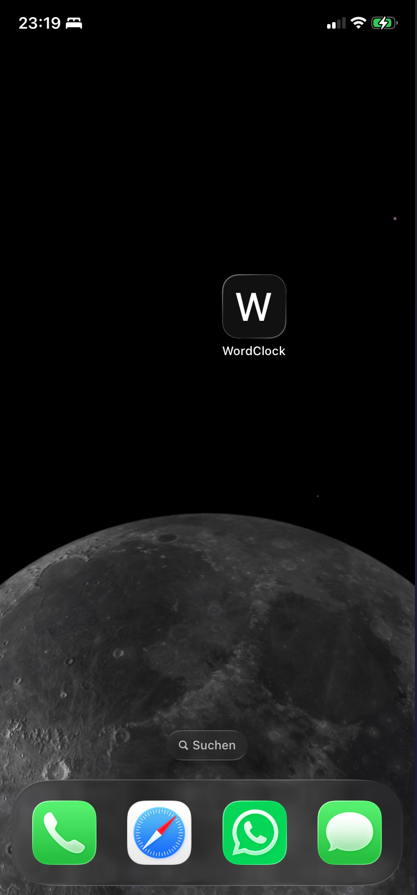
\includegraphics[width=0.37\linewidth]{inhalt/bilder/APIHomebildschirm.png}
    \caption[Die \gls{html}-\gls{ui} als Web-App auf dem Homebildschirm]{Die \gls{html}-\gls{ui} der WordClock kann als Web-App zum Homebildschirm hinzugefügt werden und ermöglicht damit einen schnellen Zugriff auf diese.}
    \label{fig:APIHomebildschirm}
\end{figure}

Nach dem Öffnen der Benutzeroberfläche werden zunächst die aktuellen Statusinformationen der WordClock angezeigt.  
Hierzu zählen unter anderem Uhrzeit, Wetterdaten, Helligkeit, Farbwerte sowie Sensorinformationen (vgl. Abb.~\ref{fig:APIParameteruebersicht}).
Im unteren Bereich der Benutzeroberfläche befinden sich die Bedienelemente.  
Über diese kann die WordClock ein- und ausgeschaltet sowie eine manuelle Aktualisierung der Wetterdaten ausgelöst werden (vgl. Abbildung~\ref{fig:APIEinAus}).
Zusätzlich können Helligkeit und Farbe der \gls{led}-Beleuchtung angepasst werden.  
Die Helligkeit wird über einen Slider eingestellt, während die Farbe über einen integrierten Farbwähler ausgewählt werden kann (vgl. Abb.~\ref{fig:APIFarbe}).

\begin{figure}[H]
  \centering
	\begin{subfigure}{0.35\textwidth}
    \centering
    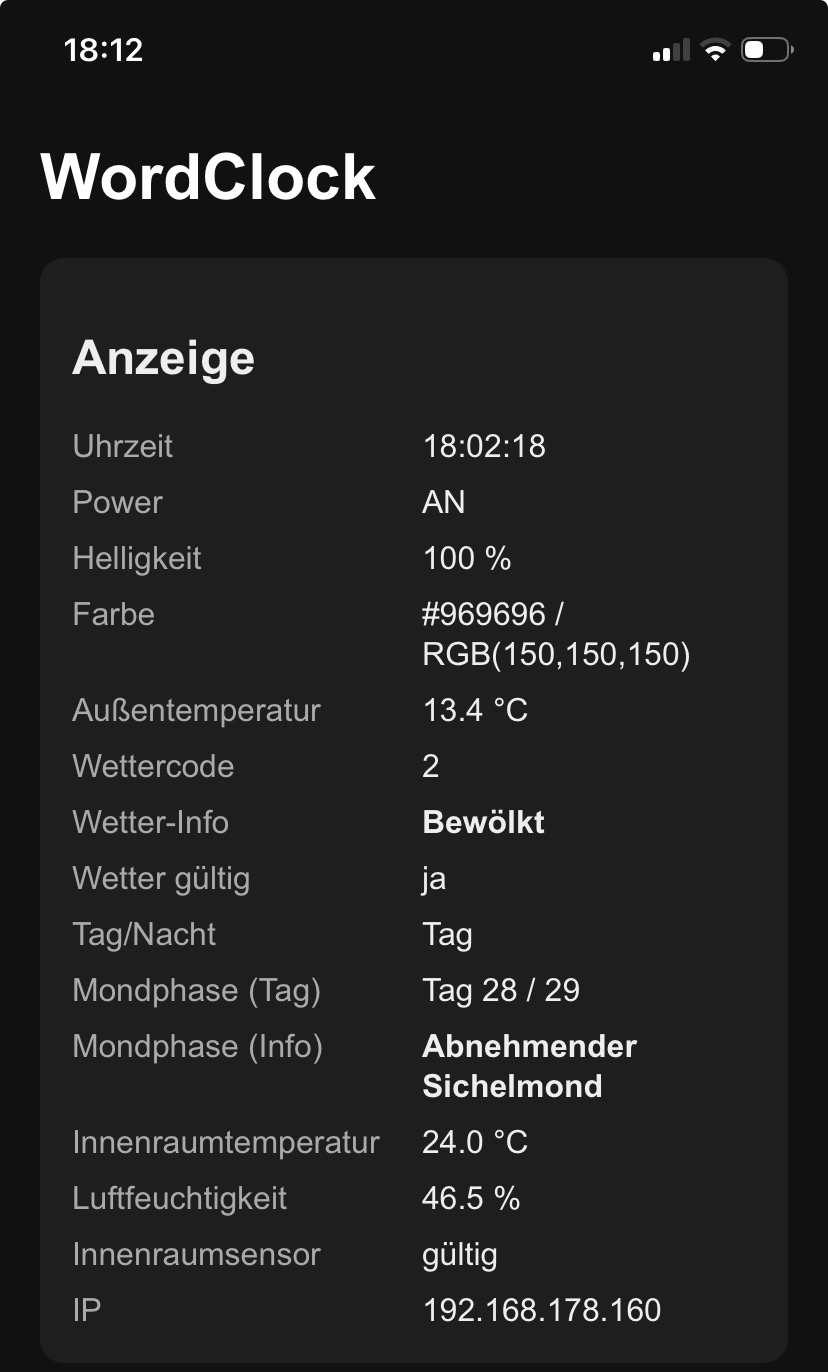
\includegraphics[width=\textwidth]{inhalt/bilder/APIParameterübersicht.png}
    \caption{Übersicht der aktuellen Systemparameter und Statusinformationen innerhalb der \gls{ui}.}
    \label{fig:APIParameteruebersicht}
	\end{subfigure}
	\hfill
	\begin{subfigure}{0.35\textwidth}
    \centering
    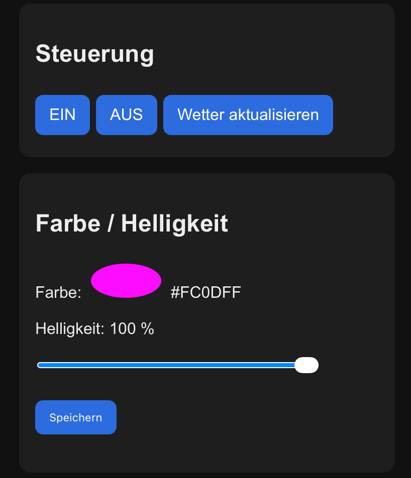
\includegraphics[width=\textwidth]{inhalt/bilder/APIEINAUSFARBE.png}
    \caption{Bedienelemente der \gls{ui} zur Steuerung der WordClock und zur Aktualisierung der Wetterinformationen.}
    \label{fig:APIEinAus}
	\end{subfigure}
  \\[1em] % Zeilenumbruch + Abstand
  \begin{subfigure}{0.35\textwidth}
    \centering
    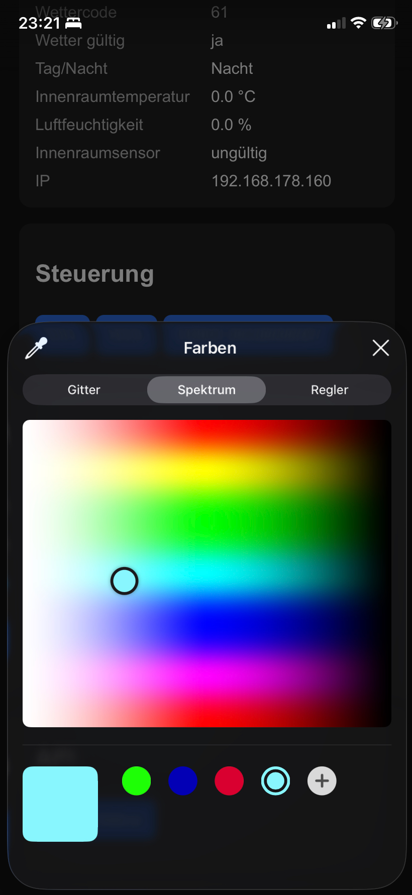
\includegraphics[width=\textwidth]{inhalt/bilder/APIFarbe.png}
    \caption{Einstellmöglichkeiten für Helligkeit und Farbe der \gls{led}-Beleuchtung innerhalb der \gls{ui}.}
    \label{fig:APIFarbe}
	\end{subfigure}
	\caption{Parameterübersicht und Funktionen in der \gls{ui}.}
\end{figure}